% This version of CVPR template is provided by Ming-Ming Cheng.
% Please leave an issue if you found a bug:
% https://github.com/MCG-NKU/CVPR_Template.

% \documentclass[review]{cvpr}
\documentclass[final]{cvpr}

\usepackage{times}
\usepackage{epsfig}
\usepackage{graphicx}
\usepackage{amsmath}
\usepackage{amssymb}

% Include other packages here, before hyperref.

% If you comment hyperref and then uncomment it, you should delete
% egpaper.aux before re-running latex.  (Or just hit 'q' on the first latex
% run, let it finish, and you should be clear).
\usepackage[pagebackref=true,breaklinks=true,colorlinks,bookmarks=false]{hyperref}


\def\confYear{CVPR 2021}
%\setcounter{page}{4321} % For final version only


\begin{document}

%%%%%%%%% TITLE
\title{The Report of the Assignment 1:\\Implementing and Reproducing Elastic Weight Consolidation}

\author{Seungmin Lee\\
Seoul National University\\
{\tt\small dltmdals14@snu.ac.kr}
}

\onecolumn
\maketitle


%%%%%%%%% BODY TEXT
\section{Introduction}
Elastic Weight Consolidation (EWC)~\cite{ewc} is a pioneering work that tackles continual learning problems. Even though many researchers have already validated EWC in their papers, we implement and reproduce EWC and compare it with L2 regularization. We conduct two experiments using CIFAR-100~\cite{cifar} and MNIST~\cite{mnist}: (a) hyperparameter searching, (b) comparing the effectiveness of EWC, L2 regularization, and no regularization. In these experiments, we learn the following three lessons. First, both regularization can alleviate \textit{catastrophic forgetting}. Second, the optimal hyperparameters can be highly different between datasets. For example, the optimal hyperparameter for CIFAR100 is 1.0. On the other hand, the optimal value is 100.0 for MNIST. Third, on simple datasets such as MNIST, EWC can be less effective than L2 regularization. 

\section{Methods}\label{method}
In this section, we summarize the methods that we implement for this assignment. Because our primary concerns are regularization-based continual learning methods, the loss functions have the same form as follows:
\begin{align}
	\mathcal{L}(\theta) = \mathcal{L}_{CE}(\theta) + \lambda\mathcal{L}_{reg}(\theta, \theta_T)
\end{align}
where $\theta$ and $\theta_T$ denote the current model weights and the previous weights after training on task $T$, repectively, and $lambda$ is the hyperparameter that balances the classification loss $\mathcal{L}_{CE}$ and the regularization loss $\mathcal{L}_{reg}$. The regularization loss term $\mathcal{L}_{reg}$ makes the difference between EWC, L2 regularization, and no regularization.

EWC alleviates catastrophic forgetting by preventing $\theta$ far away from the important weights of $\theta_{T}$ because $\theta_{T}$ encodes the knowledge for solving the previous tasks. EWC estimates the importance of each weight by calculating Fisher Information Matrix. Therefore, the regularization term of EWC~\cite{ewc} is 
\begin{align}
	\mathcal{L}_{reg}(\theta, \theta_T) = \sum_i F_i(\theta_i - \theta_{T,i})^2
\end{align}
where $F$ denotes the Fisher information matrix, $i$ is an index of each parameters. For efficiency, EWC adopts the diagonal approximation of the Fisher information matrix.

L2 regularization uses the following equation as its regularization term:
\begin{align}
	\mathcal{L}_{reg}(\theta, \theta_T) = \sum_i(\theta_i - \theta_{T,i})^2.
\end{align}
We can interpret that L2 regularization does not consider the importance of each weight. We use L2 regularization to validate whether the EWC's importance estimation is helpful or not. No regularization or vanilla training does not utilize $L_{reg}$. 

\section{Experiments}
In this section, we describe the experiment settings and their results. First, we conduct experiments for finding the optimal value of $\lambda$ used for balancing $\mathcal{L}_{CE}$ and $\mathcal{L}_{reg}$. In the second experiment, we compare the three methods described in the section~\ref{method}. We follow the provided guideline for the experiments. We use Adam optimizer~\cite{adam}, 1e-3 as the learning rate, and batch size 256 for all the experiments. We use 20 and 60 epochs for MNIST~\cite{mnist} and CIFAR-100~\cite{cifar}, respectively. 

\subsection{Hyperparameter Searching}\label{hyper_exp}
In this experiments, we search the optimal $\lambda$ for each regularization methods.
We use \{0.1, 0.5, 1.0, 10.0, 20.0, 40.0, 100.0, 200.0\} for the hyperparameters searching scope. Figure~\ref{hyper} shows the results of the experiments. The x-axis of each plot is the number of tasks learned so far, and the y-axis represents the average accuracy.  We fix the random seed as 0 for replacing another randomness. As we can observe, the smallest $\lambda$ shows the best average accuracy for L2 regularization. We can also observe that bigger $\lambda$ has detrimental effects on learning new tasks.
On the other hand, the optimal $\lambda$ for EWC varies depending on datasets. For example, the optimal $\lambda$ for CIFAR-100 is 1.0, but the optimal value for MNIST is 200.0. The large gap between the two values implies that the complexity of given tasks can affect the importance of the regularization term. Furthermore, we can observe that EWC is less sensitive to the hyperparameter. 


\begin{figure}[t]
    \centering
	\begin{tabular}{c@{\hskip0.5cm}c}
		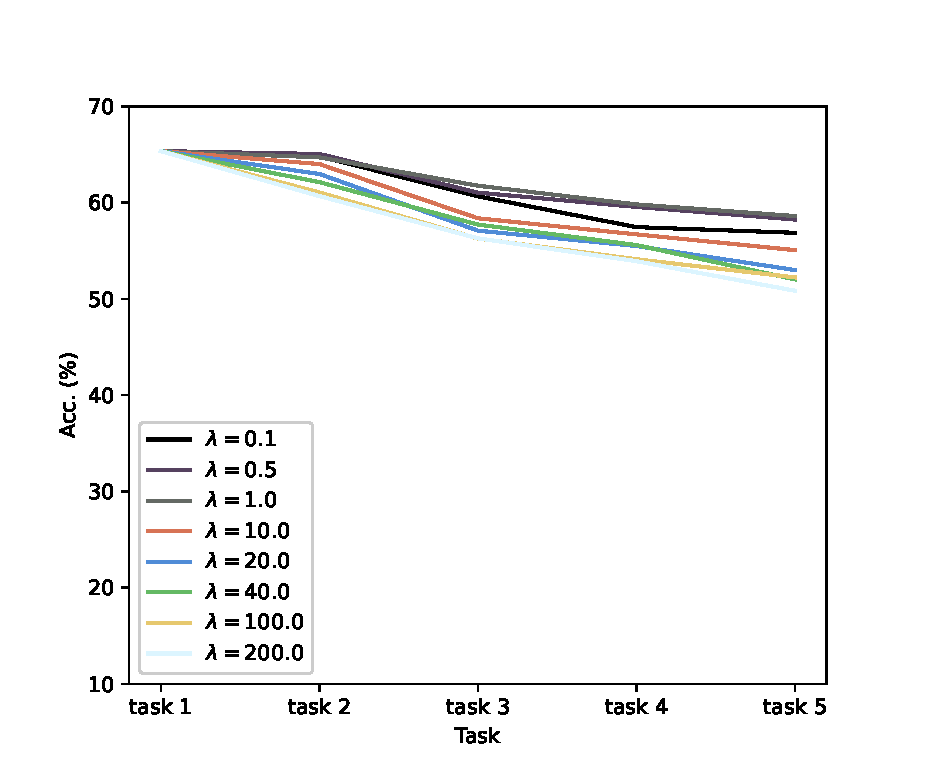
\includegraphics[width=0.45\textwidth]{resources/ewc_CIFAR.eps}&%	
        \includegraphics[width=0.45\textwidth]{resources/l2_CIFAR.eps}\\%
        (a) EWC CIFAR100 & (b) L2 CIFAR100\\
        \includegraphics[width=0.45\textwidth]{resources/ewc_MNIST.eps}&%	
        \includegraphics[width=0.45\textwidth]{resources/l2_MNIST.eps}\\%
		(c) EWC MNIST  & (d) L2 MNIST \\
	\end{tabular}\vspace{0.2cm}
	\caption{The results of the hyperparameters searching experiments. The x-axis of each plot is the number of tasks learned so far, and the y-axis represents the average accuracy.}
	% \vspace{-0.4cm}
    \label{hyper}
\end{figure}

\subsection{Comparing Regularization Methods}
Using the optimal $\lambda$ that we found in experiment~\ref{hyper_exp}, we compare the effectiveness of each regularization. As mentioned before, L2 regularization uses $\lambda=0.1$ for both datasets, and EWC uses $\lambda=1.0$ and $\lambda=200.0$ for CIFAR-100 and MNIST, respectively. We vary the random seed from 0 to 6 and average the accuracies for removing randomness. Figure~\ref{comp} displays the results of the experiments. As same as before, the x-axis represents the number of tasks learned so far, and the y-axis of each plot is the average accuracy.
For CIFAR-100 (Figure~\ref{comp} (a)), EWC shows the best performance across all the stages with a high margin. Interestingly, L2 regularization shows slightly lower performance than vanilla learning until they reach the last task, which implies that L2 regularization is too hard for learning new tasks. 
For MNIST (Figure~\ref{comp} (b)), L2 regularization exhibits better performance than EWC except for the last stage. This observation implies that EWC can be less effective when using it on a simple dataset or problem. In this experiment, the average accuracy increases after task 3 while the accuracy consistently decreases on CIFAR-100. Vanilla training shows the worst performance as we can expect.

\begin{figure}[t]
    \centering
	\begin{tabular}{c@{\hskip0.5cm}c}
		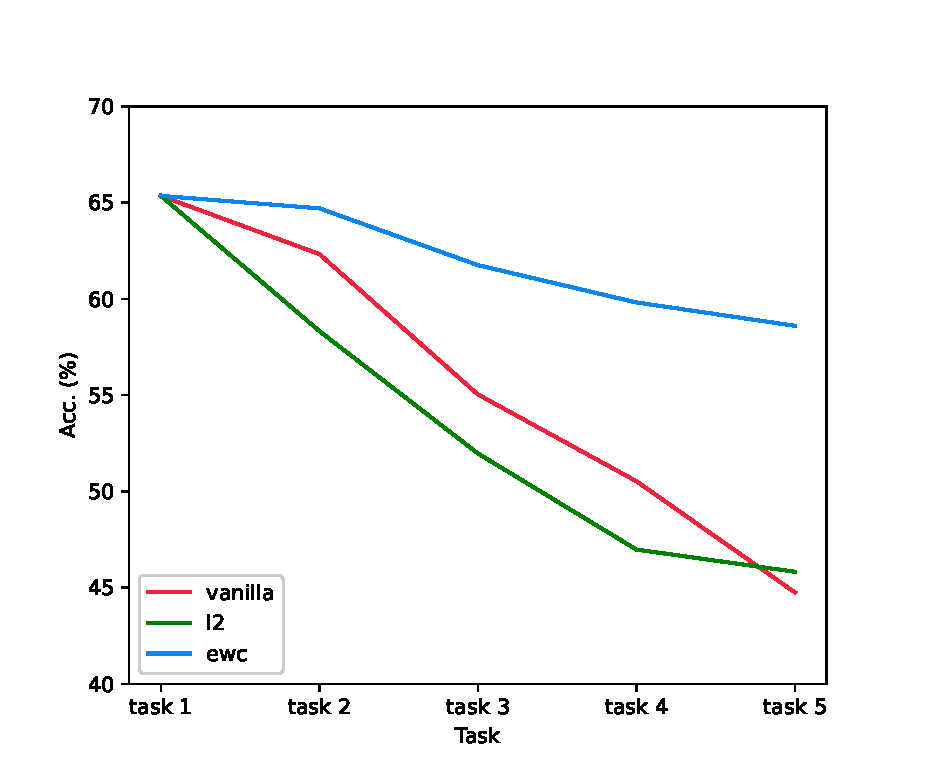
\includegraphics[width=0.45\textwidth]{resources/comp_CIFAR.eps}&%	
        \includegraphics[width=0.45\textwidth]{resources/comp_MNIST.eps}\\%
        (a) Comparing on CIFAR100 & (b) Comparing on MNIST\\
	\end{tabular}\vspace{0.2cm}
	\caption{The results of the comparison experiments. The x-axis and the y-axis represent the number of tasks learned so far and the average accuracy, respectively.}
	% \vspace{-0.4cm}
	\label{comp}
\end{figure}

\section{Conclusion}
In this assignment, we implemented EWC, a pioneering work that prevents catastrophic forgetting in continual learning. Using MNIST and CIFAR-100 datasets, we conducted hyperparameter searching experiments for finding the optimal $\lambda$ for each regularization. Using the found optimal $\lambda$, we conducted experiments for comparing the three methods (EWC, L2 regularization, and vanilla training). We found that both L2 regularization and EWC can alleviate the catastrophic forgetting. However. L2 regularization was too hard, so it can hinder the model from learning new tasks.
Moreover, we observed that the optimal hyperparameters for EWC vary depending on datasets. Finally, we observed that L2 regularization could be more effective than EWC on a simple dataset such as MNIST. These results are helpful to understand the actual effectiveness of EWC and other regularizations.


{\small
\bibliographystyle{ieee_fullname}
\bibliography{egbib}
}

\end{document}
